% Rhizome Neural Operator architecture diagram
% Build:  cd Figures/src && pdflatex rhizome_architecture.tex && mv rhizome_architecture.pdf ..
\documentclass[tikz,border=4pt]{standalone}
\usepackage[T1]{fontenc}
\IfFileExists{fourier.sty}{\usepackage{fourier}}{\usepackage{lmodern}}
\usepackage{amsmath,amssymb,bm}
\usepackage[dvipsnames]{xcolor}
\usetikzlibrary{arrows.meta,positioning,calc,fit,backgrounds}

% ---- palette (matches fno_architecture.tex / unet_architecture.tex) --
\colorlet{lift}{Gray!18}
\colorlet{fourier}{NavyBlue!14}
\colorlet{fourierline}{NavyBlue!75!black}
\colorlet{gate}{ForestGreen!16}
\colorlet{gateline}{ForestGreen!75!black}
\colorlet{val}{BurntOrange!18}
\colorlet{valline}{BurntOrange!85!black}
\colorlet{layer}{ForestGreen!6}

\begin{document}
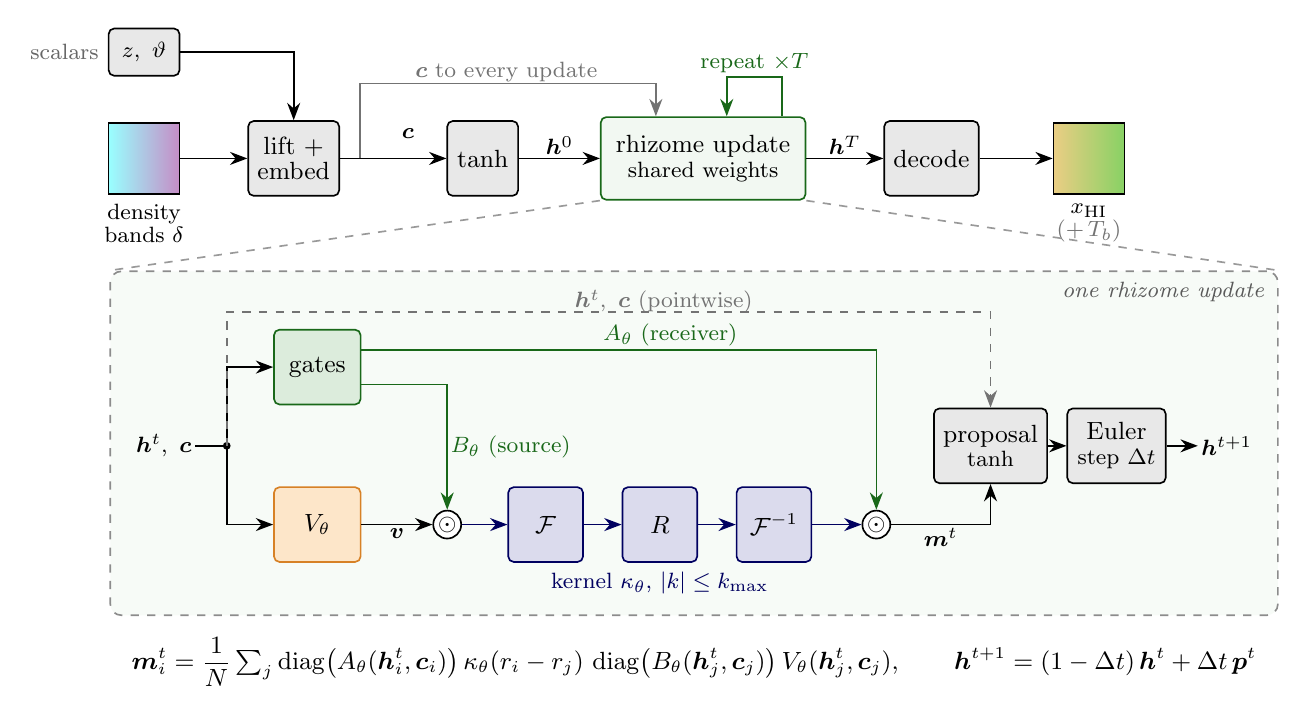
\begin{tikzpicture}[
    font=\small,
    >={Stealth[length=2.2mm]},
    every path/.style={line width=0.6pt},
    blk/.style={draw, rounded corners=2pt, minimum height=0.95cm,
                minimum width=1.1cm, align=center},
    lp/.style={blk, fill=lift},
    sp/.style={blk, fill=fourier, draw=fourierline, minimum width=0.95cm},
    gt/.style={blk, fill=gate, draw=gateline},
    vl/.style={blk, fill=val, draw=valline},
    mul/.style={draw, circle, inner sep=0.5pt, fill=white, font=\footnotesize},
    field/.style={draw, minimum size=0.9cm, inner sep=0pt},
    lab/.style={font=\footnotesize, inner sep=1pt},
  ]

  % =================== top row: full model ===========================
  \node[field, left color=Cyan!40, right color=Purple!45] (d) at (0,0) {};
  \node[lab, below=2pt of d, align=center] {density\\[-1pt] bands $\delta$};
  \node[lp, minimum width=0.9cm, minimum height=0.6cm, font=\footnotesize] (sc) at (0,1.35) {$z,\ \vartheta$};
  \node[lab, left=2pt of sc, text=black!60] {scalars};

  \node[lp] (lift) at (1.9,0) {lift +\\[-2pt] embed};
  \node[lab] (c) at (3.35,0.32) {$\bm c$};
  \node[lp, minimum width=0.9cm] (th) at (4.3,0) {$\tanh$};

  \node[blk, fill=layer, draw=gateline, minimum width=2.6cm, minimum height=1.05cm]
       (R) at (7.1,0) {rhizome update\\[-2pt] \footnotesize shared weights};
  \node[lp] (dec) at (10.0,0) {decode};

  \node[field, left color=Goldenrod!55, right color=OliveGreen!45] (x) at (12.0,0) {};
  \node[lab, below=2pt of x, align=center] {$x_{\mathrm{HI}}$\\[-1pt]\textcolor{black!55}{($+\,T_b$)}};

  \draw[->] (d) -- (lift);
  \draw[->] (sc) -| (lift);
  \draw[->] (lift) -- (th);
  \draw[->] (th) -- node[lab, above] {$\bm h^0$} (R);
  \draw[->] (R) -- node[lab, above] {$\bm h^{T}$} (dec);
  \draw[->] (dec) -- (x);

  % conditioning c is fed into every update
  \draw[->, black!55] ($(lift.east)+(0.25,0)$) -- ++(0,0.95) -| ($(R.north)+(-0.6,0)$);
  \node[lab, text=black!55] at (4.6,1.1) {$\bm c$ to every update};
  % recurrence loop
  \draw[->, draw=gateline, line width=0.8pt] ($(R.north)+(1.0,0)$) -- ++(0,0.5) -| node[lab, above, pos=0.25, text=gateline] {repeat $\times T$} ($(R.north)+(0.3,0)$);

  % =================== bottom panel: one update ======================
  \def\yU{-2.65}  % gate line
  \def\yM{-3.65}  % state line
  \def\yD{-4.65}  % value / spectral line

  \node[lab] (in) at (0.25,\yM) {$\bm h^t,\ \bm c$};
  \coordinate (split) at (1.05,\yM);

  \node[gt] (G) at (2.2,\yU) {gates};
  \node[vl] (V) at (2.2,\yD) {$V_\theta$};

  \node[mul] (m1) at (3.85,\yD) {$\odot$};
  \node[sp] (F)  at (5.1,\yD) {$\mathcal{F}$};
  \node[sp] (Rk) at (6.55,\yD) {$R$};
  \node[sp] (Fi) at (8.0,\yD) {$\mathcal{F}^{-1}$};
  \node[mul] (m2) at (9.3,\yD) {$\odot$};

  \node[lp, minimum width=1.25cm] (P) at (10.75,\yM) {proposal\\[-2pt]\footnotesize $\tanh$};
  \node[lp, minimum width=1.25cm] (E) at (12.35,\yM) {Euler\\[-2pt]\footnotesize step $\Delta t$};
  \node[lab] (out) at (13.75,\yM) {$\bm h^{t+1}$};

  \draw (in) -- (split); \fill (split) circle (1.4pt);
  \draw[->] (split) |- (G);
  \draw[->] (split) |- (V);
  % source gate -> multiply with value
  \draw[->, draw=gateline] ($(G.east)+(0,-0.22)$) -| node[lab, right, pos=0.75, text=gateline] {$B_\theta$ (source)} (m1.north);
  \draw[->] (V) -- node[lab, below] {$\bm v$} (m1);
  \draw[->, draw=fourierline] (m1) -- (F);
  \draw[->, draw=fourierline] (F) -- (Rk);
  \draw[->, draw=fourierline] (Rk) -- (Fi);
  \draw[->, draw=fourierline] (Fi) -- (m2);
  % receiver gate -> multiply after the kernel
  \draw[->, draw=gateline] ($(G.east)+(0,0.22)$) -| node[lab, above, pos=0.3, text=gateline] {$A_\theta$ (receiver)} (m2.north);
  \draw[->] (m2) -| node[lab, below, pos=0.25] {$\bm m^t$} (P.south);
  % proposal also sees h, c
  \draw[->, black!55, dashed] (split) ++(0,0.0) -- ++(0,1.7) -| (P.north);
  \node[lab, text=black!55] at (6.6,-1.82) {$\bm h^t,\ \bm c$ (pointwise)};
  \draw[->] (P) -- (E);
  \draw[->] (E) -- (out);

  \node[lab, below=2pt of Rk, text=fourierline] {kernel $\kappa_\theta$, $|k|\le k_{\max}$};

  \coordinate (fitA) at ($(Rk.south)+(0,-0.35)$);
  \coordinate (fitB) at (0,-1.75);
  \begin{scope}[on background layer]
    \node[draw=black!45, dashed, rounded corners=4pt, fill=layer!60,
          inner xsep=8pt, inner ysep=9pt,
          fit=(in) (G) (V) (Fi) (out) (P) (E) (fitA) (fitB)] (panel) {};
  \end{scope}
  \node[lab, anchor=north east, font=\footnotesize\itshape, text=black!65]
       at ($(panel.north east)+(-4pt,-3pt)$) {one rhizome update};

  \draw[black!40, dashed] (R.south west) -- (panel.north west);
  \draw[black!40, dashed] (R.south east) -- (panel.north east);

  \node[below=4pt of panel, font=\small]
       {$\bm m^t_i=\dfrac1N\sum_j \operatorname{diag}\!\big(A_\theta(\bm h^t_i,\bm c_i)\big)\,
        \kappa_\theta(r_i-r_j)\,\operatorname{diag}\!\big(B_\theta(\bm h^t_j,\bm c_j)\big)\,V_\theta(\bm h^t_j,\bm c_j),
        \qquad \bm h^{t+1}=(1-\Delta t)\,\bm h^t+\Delta t\,\bm p^t$};
\end{tikzpicture}
\end{document}
